\documentclass[11pt]{amsart}
\usepackage[margin=2.6cm]{geometry}
\usepackage{amssymb,amsmath,tikz,booktabs}
\usepackage[hidelinks]{hyperref}
\newtheorem{theorem}{Theorem}
\newtheorem{corollary}[theorem]{Corollary}
\newtheorem{lemma}[theorem]{Lemma}
\newtheorem{proposition}[theorem]{Proposition}
\newtheorem{conjecture}[theorem]{Conjecture}
\theoremstyle{remark}\newtheorem{remark}[theorem]{Remark}
\newcommand{\R}{\mathbb{R}}
\newcommand{\Prob}{\mathbb{P}}
\newcommand{\E}{\mathbb{E}}
\DeclareMathOperator{\Vol}{Vol}
\DeclareMathOperator{\area}{area}
\DeclareMathOperator{\width}{width}

\title{Does the smallest enclosing copy fit?\\ Random points in a convex polygon}
\author{Vamshi Jandhyala}
\date{Preprint, version 1, 8 October 2026. Not peer reviewed.}
\subjclass[2020]{60D05; 52A22; 60G55}
\keywords{random polygons, smallest enclosing copy, Poisson limit, linear programming, Mecke equation, formal verification}

\begin{document}
\begin{abstract}
Choose $n$ independent uniform points in a convex polygon $K$ and let $Q_n$ be a smallest similar copy of $K$, of any
orientation, that contains them all. We show that the probability that $Q_n$ can be chosen inside $K$ converges, as
$n\to\infty$, to an explicit constant $p(K)$, and we give a formula for $p(K)$ as an integral over a Poisson limit
model. For an equilateral triangle $p=13/48$ and for a square $p=1/4$; numerically, $p$ ranges over $[13/48,25/72)$ for
triangles, and we conjecture that the equilateral triangle is the minimiser. For regular $q$-gons the constants
are not monotone in $q$ (the computed values for $q=5,7$ lie below their even neighbours) and appear to settle near $0.146$ (computed up to $q=200$), far from the value $1/2$
that a Mathematics Stack Exchange answer establishes for the disk. The answer is
governed by the freedom to rotate the enclosing copy, which has no analogue for the disk.
\end{abstract}
\maketitle

\noindent\emph{Status of this preprint.} Every theorem, lemma and corollary is formally verified in Lean~4
(Section~\ref{sec:lean}), using only Lean's standard axioms. The exposition, the numerical results of
Section~\ref{sec:num} and Conjecture~\ref{conj:eq} are not formally verified, and this version has not yet been
independently reviewed.


\section{Introduction}

Drop $n$ random points into a disk and draw the smallest circle containing them. Does that circle lie inside the
disk? A question on Mathematics Stack Exchange \cite{mse} asked for the limiting probability, and an answer there
shows that it is exactly $1/2$. A follow-up on MathOverflow \cite{mo} asked whether the same holds when the disk and
the circle are replaced by a regular polygon and a smallest enclosing regular polygon of the same kind, which may be
rotated. The asker's simulations for two points suggested a family resemblance with the disk.

The answer is no, and the reason is instructive. A smallest enclosing polygon wants to turn slightly: turning by an
angle of order $1/n$ lets it hug the outermost points better, and the same turn pushes its corners out by a distance
of order $1/n$, the same order as the gaps between the outermost points and the sides. Whether the copy fits is
decided by a competition between these two effects, and it can be computed exactly.

\begin{figure}[ht]
\centering
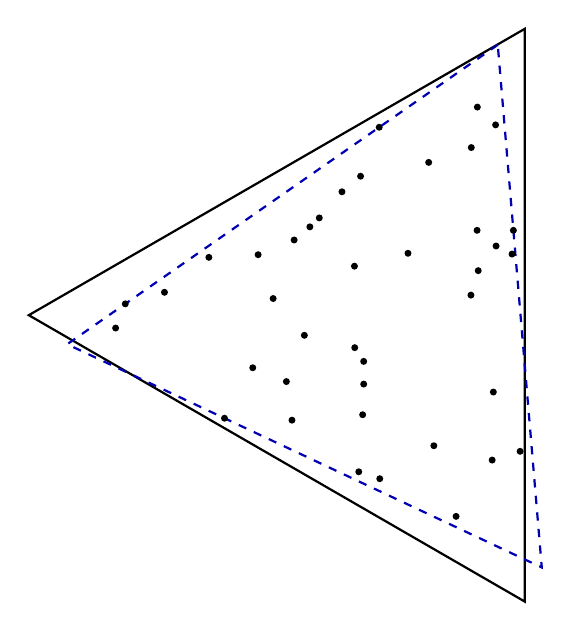
\begin{tikzpicture}[scale=2.1]
\draw[thick] (1.0000,1.7321) -- (-2.0000,0.0000) -- (1.0000,-1.7321) -- cycle;
\draw[blue!70!black, dashed, thick] (0.8362,1.6350) -- (-1.7677,-0.1757) -- (1.1024,-1.5254) -- cycle;
\fill (0.7111,0.5133) circle (0.6pt);
\fill (-0.3952,0.4548) circle (0.6pt);
\fill (0.9224,0.3697) circle (0.6pt);
\fill (0.4185,0.9240) circle (0.6pt);
\fill (-0.8164,-0.6231) circle (0.6pt);
\fill (-0.3000,0.5343) circle (0.6pt);
\fill (-0.3334,-0.1217) circle (0.6pt);
\fill (-0.9108,0.3499) circle (0.6pt);
\fill (-1.1794,0.1384) circle (0.6pt);
\fill (0.6741,0.1215) circle (0.6pt);
\fill (0.9307,0.5130) circle (0.6pt);
\fill (0.9713,-0.8232) circle (0.6pt);
\fill (-0.4083,-0.6349) circle (0.6pt);
\fill (-0.0305,0.2965) circle (0.6pt);
\fill (-0.6131,0.3657) circle (0.6pt);
\fill (0.7127,1.2585) circle (0.6pt);
\fill (-0.0287,-0.1964) circle (0.6pt);
\fill (-0.6455,-0.3179) circle (0.6pt);
\fill (0.8095,-0.4647) circle (0.6pt);
\fill (0.0255,-0.4167) circle (0.6pt);
\fill (0.2933,0.3744) circle (0.6pt);
\fill (0.7180,0.2693) circle (0.6pt);
\fill (0.4498,-0.7895) circle (0.6pt);
\fill (0.0065,0.8405) circle (0.6pt);
\fill (0.8024,-0.8761) circle (0.6pt);
\fill (-0.0044,-0.9471) circle (0.6pt);
\fill (-0.5222,0.1008) circle (0.6pt);
\fill (0.6761,1.0138) circle (0.6pt);
\fill (-0.4421,-0.4014) circle (0.6pt);
\fill (0.8232,1.1509) circle (0.6pt);
\fill (0.0191,-0.6020) circle (0.6pt);
\fill (-1.4163,0.0687) circle (0.6pt);
\fill (0.1226,-0.9889) circle (0.6pt);
\fill (-1.4748,-0.0777) circle (0.6pt);
\fill (0.1193,1.1365) circle (0.6pt);
\fill (0.0254,-0.2793) circle (0.6pt);
\fill (0.5841,-1.2166) circle (0.6pt);
\fill (-0.2432,0.5883) circle (0.6pt);
\fill (0.8260,0.4184) circle (0.6pt);
\fill (-0.1059,0.7463) circle (0.6pt);
\end{tikzpicture}

\caption{Forty uniform points in an equilateral triangle (solid). The smallest enclosing equilateral triangle
(dashed) is rotated by about $0.08$ radians and pokes out across the right side, near the lower right corner, although it is smaller than the
outer triangle.}
\label{fig:example}
\end{figure}

\subsection*{Results}
Let $K$ be a convex polygon and $X_1,\dots,X_n$ independent uniform points in $K$. A \emph{copy} of $K$ is a set
$\lambda R_\theta K+c$ with $\lambda>0$, $R_\theta$ a rotation and $c\in\R^2$. Let $E_n$ be the event that some copy of
minimal $\lambda$ containing all $X_j$ lies in $K$.

\begin{theorem}\label{thm:main}
$\Prob(E_n)$ converges to the probability $p(K)$ of the event $E$ of the limit model of Section~\ref{sec:model}, and
$p(K)$ is given by the formula of Theorem~\ref{thm:formula}.
\end{theorem}

\begin{corollary}[Triangles]\label{cor:tri}
For a triangle with sides $L_1,L_2,L_3$,
\[
p=\frac{1}{2\sum_i L_i^2}\sum_{k=1}^{3}L_k^2\,g\!\left(\frac{L_i^2}{L_k^2},\frac{L_j^2}{L_k^2}\right),\qquad
g(\alpha,\beta)=\E\big[(1-(\alpha U_1+\beta U_2)^2)_+\big],
\]
where $\{i,j,k\}=\{1,2,3\}$ and $U_1,U_2$ are independent and uniform on $[-1,1]$. In particular $p=13/48$ for the
equilateral triangle, $7/24$ for the right isosceles triangle and $29/96$ for the $30$-$60$-$90$ triangle;
$p\to 1/3$ for thin right triangles and for needle-shaped isosceles triangles (apex angle tending to $0$), and
$p\to25/72$ for flat isosceles triangles (apex angle tending to $\pi$).
\end{corollary}

\begin{corollary}[Regular polygons]\label{cor:reg}
For the regular $q$-gon,
\[
p_q=q\tan\frac{\pi}{q}\;\E\big[\Vol(T)\,\mathbf 1\{0\in\operatorname{int}T\}\big]+\mathbf 1\{q\text{ even}\}\,\frac{8}{3q^2},
\]
where $T$ is the tetrahedron spanned by four independent points, each chosen by picking one of the $q$ vertical edges
of the prism $P_q\times[-1,1]$ uniformly at random ($P_q$ the regular $q$-gon inscribed in the unit circle) and a
uniform height on it. In particular $p_3=13/48$ and $p_4=1/4$ (Section~\ref{sec:reg}), and numerically $p_q$ is
close to $0.146$ for large $q$ (Table~\ref{tab:reg}).
\end{corollary}

\begin{conjecture}\label{conj:eq}
Among all triangles, $p$ is minimised by the equilateral triangle; the range of $p$ over triangles is $[13/48,25/72)$.
\end{conjecture}

The formula of Corollary~\ref{cor:tri} is explicit enough to evaluate on a fine grid: over $28{,}800$ triangle shapes
the minimum is attained at the equilateral triangle and $p$ increases away from it (Section~\ref{sec:num}).

The limit model is a Poisson process along each side, as in Groeneboom's study of convex hulls of uniform samples
from a polygon \cite{groeneboom88,groeneboom12}, but at a different scale: the relevant points lie within distance
$O(1/n)$ of the sides along their whole length, not near the vertices. Uniform samples from polygons are also the
setting of Sylvester's problem, the probability that the $n$ points are in convex position, whose asymptotics Morin
obtained for regular \cite{morin25} and for general convex polygons \cite{morin26}; that event depends on the whole
sample, whereas $E_n$ depends only on the points within distance $O(1/n)$ of the boundary.

\section{The limit model}\label{sec:model}

Fix the polygon $K$, scaled to area $1$, with sides $1,\dots,m$. Side $i$ has outward unit normal $u_i$, support
number $h_i$ (with the origin inside $K$), tangent $t_i=R_{90^\circ}u_i$, and is the set of points $x$ with
$x\cdot u_i=h_i$ and $s=x\cdot t_i\in[a_i,b_i]$; its length is $L_i=b_i-a_i$. Two identities are used repeatedly:
\begin{equation}\label{eq:ids}
\sum_i L_iu_i=0,\qquad \sum_i L_ih_i=2,\qquad \sum_i L_ib_i=\tfrac12\sum_iL_i^2=-\sum_iL_ia_i .
\end{equation}
The last holds because $L_i(a_i+b_i)/2=(b_i^2-a_i^2)/2$ and $b_i^2-a_i^2=|v_{i+1}|^2-|v_i|^2$ telescopes over the
vertices $v_i$.

\subsection*{Heuristic} A point $x$ at depth $d=h_i-x\cdot u_i$ below side $i$ and position $s=x\cdot t_i$ has
support $x\cdot R_\theta u_i=h_i-d+\theta s+O(\theta^2)$ in the rotated normal direction. A copy $(1+\varepsilon)R_\theta
K+c$ has support $(1+\varepsilon)h_i+c\cdot u_i+O(\theta|c|)$ in the same direction, and its vertex at the end of side
$i$ pokes out across the line of side $i$ unless $\varepsilon h_i+c\cdot u_i\le\min(\theta a_i,\theta b_i)$. With
$\Theta=n\theta$, $C=nc$, $D=nd$ and $\varepsilon$ replaced by $n\varepsilon$, all quantities are of order one.

\begin{figure}[ht]
\centering
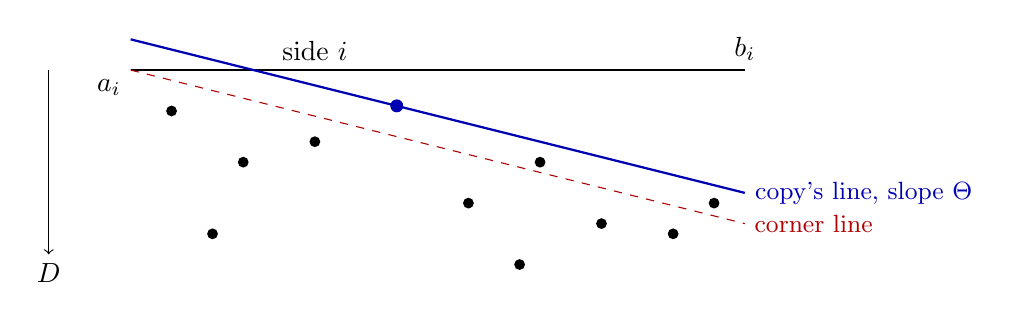
\begin{tikzpicture}[scale=1.3]
\draw[thick] (-3,0) -- (3,0);
\node[above] at (-1.2,0) {side $i$};
\draw[->] (-3.8,0) -- (-3.8,-1.8) node[below] {$D$};
\node[below left] at (-3,0) {$a_i$}; \node[above] at (3,0) {$b_i$};
\draw[red!70!black,dashed] (-3,0) -- (3,-1.5) node[right] {\small corner line};
\draw[blue!70!black,thick] (-3,0.3) -- (3,-1.2) node[right] {\small copy's line, slope $\Theta$};
\foreach \x/\y in {-2.6/-0.4,-1.9/-0.9,-1.2/-0.7,0.3/-1.3,1.0/-0.9,1.6/-1.5,2.3/-1.6,2.7/-1.3,-2.2/-1.6,0.8/-1.9}
  \fill (\x,\y) circle (1.5pt);
\fill[blue!70!black] (-0.4,-0.35) circle (1.8pt);
\end{tikzpicture}
\caption{The limit model on one side, drawn with depth $D$ downwards. The copy's side corresponds to the solid line
$D=\Theta s-H_i$; every point must lie on or below it (deeper), which is $H_i\ge M_i(\Theta)$, and the marked point is
tight. The copy fits at the end $a_i$ when its line lies on or below the dashed corner line $D=\Theta(s-a_i)$; here it
lies above, so the copy pokes out at that corner.}
\label{fig:model}
\end{figure}

\subsection*{Definition}
Let $\Pi_1,\dots,\Pi_m$ be independent Poisson processes of intensity $1$ on the strips $[a_i,b_i]\times[0,\infty)$,
and $M_i(\Theta)=\sup_{(s,D)\in\Pi_i}(\Theta s-D)$. The \emph{limit LP} is
\[
\text{minimise }\varepsilon\quad\text{over }(\varepsilon,C,\Theta)\in\R\times\R^2\times\R\quad\text{subject to}\quad
H_i:=\varepsilon h_i+C\cdot u_i\ \ge\ M_i(\Theta)\ \ (i=1,\dots,m),
\]
and $E$ is the event that some optimal $(\varepsilon,C,\Theta)$ satisfies $H_i\le\min(\Theta a_i,\Theta b_i)$ for
all $i$. The model is scale free: changing the intensity rescales $D,\varepsilon,C,\Theta$ together and leaves $E$
unchanged.

\begin{lemma}\label{lem:exist}
Almost surely each $M_i$ is finite, convex and piecewise linear, and the optimal set $Z^*$ of the limit LP is nonempty
and compact.
\end{lemma}

\begin{proof}
Each strip contains only finitely many points with $D\le T$ for every $T$. On $|\Theta|\le B$, fix any point
$(s_0,D_0)$ of $\Pi_i$; since $|s|\le S_i:=\max(|a_i|,|b_i|)$, every point with $D>D_0+2BS_i$ has $\Theta s-D<\Theta
s_0-D_0$ for all such $\Theta$, so only the finitely many points with $D\le D_0+2BS_i$ can contribute, and $M_i$ is a
maximum of finitely many affine functions on any bounded $\Theta$-interval. The point $z=0$ is feasible, since $M_i(0)=-\inf D\le0$, so
$\varepsilon^*\le0$. By \eqref{eq:ids}, $\sum_iL_iH_i=2\varepsilon$ for every $(\varepsilon,C,\Theta)$, so feasibility gives
$2\varepsilon\ge F(\Theta):=\sum_iL_iM_i(\Theta)$. Fix $\delta>0$ with $\delta\,\mathrm{per}(K)<\tfrac14\sum_iL_i^2$
and, on each side, a point with $s\ge b_i-\delta$ and a point with $s\le a_i+\delta$. For $\Theta>0$ the first kind give
$F(\Theta)\ge\Theta(\sum_iL_ib_i-\delta\,\mathrm{per}(K))-O(1)\ge\frac\Theta4\sum_iL_i^2-O(1)$ by \eqref{eq:ids}, and
for $\Theta<0$ the second kind give the same with $|\Theta|$. Hence $\{\varepsilon\le0\}$ forces $|\Theta|$ bounded, and
$\varepsilon$ is bounded below there. For such $(\varepsilon,\Theta)$ each $C\cdot u_i=H_i-\varepsilon h_i$ is bounded
below; since $\sum_iL_i\,C\cdot u_i=0$ with all $L_i>0$, each is also bounded above, and the $u_i$ span $\R^2$, so $C$ is
bounded. The feasible set intersected with $\{\varepsilon\le0\}$ is therefore closed, bounded and nonempty, and the
minimum of $\varepsilon$ over it is attained on a compact set.
\end{proof}

\section{Convergence}\label{sec:conv}

The proof compares the finite problem with the limit model on the same marked points near the boundary. Three facts
make the comparison exact rather than approximate. First, in tangent coordinates (Lemma~\ref{lem:tangent}) the
constraint that a copy contains a sample point is exactly the constraint of the limit LP; the nonlinearity moves into
the objective, the physical scale of the copy. Second, at a nondegenerate optimum of the limit LP the tilt is
controlled by the excess of $\varepsilon$, so for large $n$ the physical scale and $\varepsilon$ have the same minimisers
over the common feasible set (Lemma~\ref{lem:stab}). Third, the fit condition of the finite problem is that of the limit
model plus a term of order $1/n$, which cannot change the outcome when the limit optimum fits strictly or fails
strictly, and almost surely one of the two happens (Lemma~\ref{lem:nondeg}). The probabilistic input is a Poisson
approximation of the points near the boundary in total variation, uniformly over events (Step~3).

\emph{Notation.} The event $E_n$ is invariant under similarities, so $K$ has area $1$; we list its vertices
counterclockwise in strictly convex position (a vertex at which the boundary is straight can be deleted). Fix
$r,R_K$ with $B(0,r)\subseteq K\subseteq B(0,R_K)$, and write $S_K=\max_i\max(|a_i|,|b_i|)$, $h_{\max}=\max_ih_i$,
$Q=\sum_iL_ib_i=\frac12\sum_iL_i^2$ and $\mathrm{per}=\sum_iL_i$. For $x\in K$ and a side $i$ let $d_i(x)=h_i-x\cdot
u_i\ge0$ be its depth and $s_i(x)=x\cdot t_i$ its position. Throughout, $q=1/n$.

\emph{Tangent coordinates.} For $z=(\varepsilon,C,\Theta)\in\R\times\R^2\times\R$ with $1+q\varepsilon>0$ let
\[
\sigma_{q,z}(x)=\frac{1}{1+q^2\Theta^2}\,T_{q\Theta}\big((1+q\varepsilon)x+qC\big),\qquad T_\tau(w)=w+\tau R_{90^\circ}w .
\]
Since $T_\tau=\sqrt{1+\tau^2}\,R_{\arctan\tau}$, the map $\sigma_{q,z}$ is a similarity with rotation angle
$\arctan(q\Theta)$ and scale
\[
\lambda_q(z)=\frac{1+q\varepsilon}{\sqrt{1+q^2\Theta^2}},
\]
and every similarity with positive scale and rotation angle in $(-\pi/2,\pi/2)$ is $\sigma_{q,z}$ for exactly one such
$z$. We call $\sigma_{q,z}(K)$ the copy $z$.

\begin{lemma}\label{lem:tangent}
Let $1+q\varepsilon>0$ and write $H_i=\varepsilon h_i+C\cdot u_i$.
\begin{itemize}
\item[(a)] A point $x$ lies in the copy $z$ if and only if, for every side $i$,
\begin{equation}\label{eq:contain}
x\cdot u_i+q\Theta\,x\cdot t_i\ \le\ (1+q\varepsilon)h_i+q\,C\cdot u_i .
\end{equation}
For a point at depth $d_i(x)=D/n$ and position $s=s_i(x)$ this is $D\ge\Theta s-H_i$, the constraint of the limit LP.
\item[(b)] There is $r_K>0$, depending only on the angles of $K$, such that if $|q\Theta|\le r_K$ the copy $z$ lies in
$K$ if and only if, for every side $i$ and $s\in\{a_i,b_i\}$,
\[
\phi_{q,i,s}(z):=\Theta s-H_i+q\big(\varepsilon\Theta s+\Theta\,C\cdot t_i+\Theta^2h_i\big)\ \ge\ 0 .
\]
At $q=0$ this is the condition $H_i\le\min(\Theta a_i,\Theta b_i)$ that defines $E$.
\end{itemize}
\end{lemma}

\begin{proof}
(a) Since $T_{-\tau}T_\tau=(1+\tau^2)\,\mathrm{id}$, the inverse of $\sigma_{q,z}$ is $x\mapsto(1+q\varepsilon)^{-1}
(T_{-q\Theta}x-qC)$, and $y\in K$ if and only if $y\cdot u_i\le h_i$ for all $i$. As $(R_{90^\circ}x)\cdot
u_i=-x\cdot t_i$, we have $T_{-\tau}x\cdot u_i=x\cdot u_i+\tau\,x\cdot t_i$, which gives \eqref{eq:contain}. Substituting
$x\cdot u_i=h_i-D/n$ and $x\cdot t_i=s$ and multiplying by $n$ gives $D\ge\Theta s-H_i$.
(b) The copy is a convex polygon whose sides are those of $K$ turned by $\arctan(q\Theta)$. If this angle is less than
half the least exterior angle of $K$, the support of the copy in the direction $u_i$ is attained at an endpoint of its
side $i$, so the copy lies in $K$ if and only if both endpoints of its side $i$ satisfy $y\cdot u_i\le h_i$, for every
$i$. The endpoint $h_iu_i+st_i$ of side $i$ is mapped to $y$ with
$(1+q^2\Theta^2)\,y\cdot u_i=(1+q\varepsilon)h_i+qC\cdot u_i-q\Theta\big((1+q\varepsilon)s+qC\cdot t_i\big)$, and
$y\cdot u_i\le h_i$ is $\phi_{q,i,s}(z)\ge0$ after dividing by $q$.
\end{proof}

So the finite problem and the limit LP share their constraints. The finite problem minimises $\lambda_q(z)$, which is
$1+q\varepsilon+O(q^2)$ on bounded sets, and its fit condition is $\phi_q\ge0$, which is the limit condition up to
$O(q)$.

\begin{proof}[Proof of Theorem~\ref{thm:main}]
\emph{Step 0: the rotation localises.} Let $\Lambda(S,\theta)$ be the least $\lambda$ with $S\subseteq\lambda
R_\theta K+c$ for some $c$. Two facts about it. First, if $S'\subseteq S+B(0,\delta)$ then
$\Lambda(S',\theta)\le\Lambda(S,\theta)+\delta/r$, because $B(0,\delta)\subseteq(\delta/r)R_\theta K$ and $\lambda
A+\mu A=(\lambda+\mu)A$ for convex $A$. Second, since $|R_{\theta'}x-R_\theta x|\le R_K|\theta-\theta'|$ on $K$, we have
$R_{\theta'}K\subseteq R_\theta K+B(0,R_K|\theta-\theta'|)\subseteq(1+R_K|\theta-\theta'|/r)R_\theta K$, so
$\theta\mapsto\Lambda(S,\theta)$ is continuous. Let $G_K$ be the finite group of angles $g$ with $R_gK=K+t_g$ for some
$t_g$. If $K\subseteq\lambda R_\theta K+c$ then $1\le\lambda^2$ by area, and $\lambda=1$ forces $K=R_\theta K+c$ (a
convex body strictly inside another has strictly smaller area), so $\Lambda(K,\theta)\ge1$ with equality only on
$G_K$. Fix $\eta>0$ with $\tan\eta\le\min(r_K,Q/4)$ and smaller than half the least gap between elements of $G_K$; by
continuity and compactness there is $\beta>0$ with $\Lambda(K,\theta)\ge1+\beta$ whenever $\theta$ is at distance at
least $\eta$ from $G_K$. Cover $K$ by finitely many balls $B(y_k,\delta/2)$, $y_k\in K$, with $\delta=\beta r/2$; each
meets $K$ in positive area, so with probability tending to $1$ each contains a sample point, and then $K\subseteq
S+B(0,\delta)$. On that event $\Lambda(S,\theta)\ge1+\beta/2>1\ge\Lambda(S,0)$ for every such $\theta$, so every
smallest copy has its rotation within $\eta$ of $G_K$. For $g\in G_K$ we have $\lambda R_{\theta+g}K+c=\lambda
R_\theta K+c+\lambda R_\theta t_g$, so rotations $\theta$ and $\theta+g$ give the same family of sets. Hence every
smallest copy is a copy $z$ with $|q\Theta|\le\tan\eta$, and it has scale $\lambda_q(z)\le1$ because $K$ itself
contains the sample.

\emph{Step 1: witnesses confine the copies.} Let $\delta_K=Q/(2\,\mathrm{per})$ and, for each side, take the windows
$W_i^+=\{x:s_i(x)\in[b_i-w_i,b_i-w_i/2]\}$ and $W_i^-=\{x:s_i(x)\in[a_i+w_i/2,a_i+w_i]\}$ near its two ends, with
$w_i=\min(\delta_K,L_i)/2$. Call points of the sample in $W_i^\pm$ at depth $d_i\le y/n$ \emph{witnesses}. The part of
$W_i^\pm$ at depth at most $y/n$ has area $w_iy/(2n)$, so the probability that some window has no witness is at most
$2m\max_i(1-w_iy/(2n))^n\le2me^{-\min_iw_iy/2}$, small for large $y$, uniformly in $n$.

Suppose every side has witnesses $x_i^\pm$ at scaled depths $D_i^\pm=nd_i(x_i^\pm)\le M$, and let $z$ satisfy their
constraints, with $\lambda_q(z)\le1$ and $|q\Theta|\le Q/4$. By Lemma~\ref{lem:tangent}(a), $D_i^+\ge\Theta s_i^+-H_i$.
Multiply by $L_i$ and sum: the terms in $C$ cancel because $\sum_iL_iu_i=0$, and $\sum_iL_ih_i=2$, so
$\Theta\sum_iL_is_i^+\le2\varepsilon+\sum_iL_iD_i^+$. Here $\sum_iL_is_i^+\ge\sum_iL_i(b_i-\delta_K)=Q/2$ by
\eqref{eq:ids}, and $\lambda_q(z)\le1$ gives $1+q\varepsilon\le\sqrt{1+q^2\Theta^2}\le1+q^2\Theta^2/2$, so
$\varepsilon\le q\Theta^2/2\le Q|\Theta|/8$. For $\Theta>0$ this yields $\Theta Q/4\le M\,\mathrm{per}$, and the
witnesses $x_i^-$ give the same bound for $\Theta<0$. With $|\Theta|$ bounded, the same sum bounds $\varepsilon$ below,
each $C\cdot u_i=H_i-\varepsilon h_i\ge\Theta s_i^+-D_i^+-\varepsilon h_i$ is bounded below, hence also above since
$\sum_iL_i\,C\cdot u_i=0$, and two of the $u_i$ are not parallel, so $C$ is bounded. So there is $R=R(M,K)$ such that
every such $z$ lies in the box $B_R=\{|\varepsilon|,|C_1|,|C_2|,|\Theta|\le R\}$, for every $n$. The same argument,
with $\varepsilon\le0$ in place of $\lambda_q(z)\le1$, shows that every $z$ feasible for the witnesses in the limit LP
with $\varepsilon\le0$ lies in $B_R$.

\emph{Step 2: only the boundary window matters.} There is $T_c=T_c(R,K)$ with $\Theta s_i(x)-H_i\le T_c$ for every
$x\in K$, $z\in B_R$ and side $i$. So, by Lemma~\ref{lem:tangent}(a), a point with $nd_i(x)>T_c$ satisfies the side-$i$
constraint of every copy in $B_R$. Fix $T\ge T_c$. Let $\mathcal O_n$ be the set of points of $K$ within $T/n$ of two
sides; it has area $O(T^2/n^2)$, so with probability tending to $1$ it contains no sample point. Mark each sample point
$x$ with $d_i(x)\le T/n$ by $(i,s_i(x),nd_i(x))$, and let $\mu_n$ be the resulting configuration. For a configuration
$\mu$ let $\mathcal G(\mu)\subseteq B_R$ be the set of copies in $B_R$ satisfying the constraints $D\ge\Theta s-H_i$
of all its marks, and define the events
\begin{align*}
F_n(\mu)&:\ \mu\text{ has witnesses at depth}\le M\text{, and some minimiser of }\lambda_q\text{ over }\mathcal
G(\mu)\\&\phantom{:\ }\text{satisfies }\phi_q\ge0,\\
F(\mu)&:\ \mu\text{ has witnesses at depth}\le M\text{, and some minimiser of }\varepsilon\text{ over }\mathcal
G(\mu)\\&\phantom{:\ }\text{satisfies }H_i\le\min(\Theta a_i,\Theta b_i)\text{ for all }i .
\end{align*}
Let $\mathcal A_n$ be the event that the $\delta$-net of Step 0 is hit, that every side has witnesses at depth at most
$y/n\le M/n$, and that no sample point lies in $\mathcal O_n$. On $\mathcal A_n$, and for $n>R/r_K$ (so that
$1+q\varepsilon>0$ and $|q\Theta|\le r_K$ on $B_R$), $E_n$ holds if and only if $F_n(\mu_n)$ holds. Indeed, by Step 0 every smallest copy is a copy $z$ with $|q\Theta|\le\tan\eta$ and
$\lambda_q(z)\le1$, so by Step 1 it lies in $B_R$, and the smallest copies are the minimisers of $\lambda_q$ over the copies in $B_R$
containing the sample; a copy in $B_R$ contains the sample if and only if it lies in
$\mathcal G(\mu_n)$, because the constraints of a point for sides it is not within $T/n$ of are slack (Step 2) and the
others are exactly the constraints of its marks (Lemma~\ref{lem:tangent}(a)); and the fit condition is $\phi_q\ge0$ by
Lemma~\ref{lem:tangent}(b). Both events are measurable: ``some minimiser of a continuous
function over a compact set lies in a closed set'' is a projection along a compact factor.

\emph{Step 3: the boundary window is Poisson.} Let $\Pi^T$ be the limit model truncated at depth $T$: independent
Poisson processes of intensity $1$ on the rectangles $[a_i,b_i]\times[0,T]$. Then
\[
\sup_F\big|\Prob(F(\mu_n))-\Prob(F(\Pi^T))\big|\to0,
\]
the supremum over all measurable events $F$ of configurations. The set of points of $K$ within $T/n$ of the sides has
area $\mathrm{per}\,T/n+O(T^2/n^2)$, so the number of sample points in it is binomial with mean
$\mathrm{per}\,T+O(1/n)$, and its law tends in total variation to the Poisson law with mean $\mathrm{per}\,T$ (the law
of rare events). Given this number, the points are independent and uniform on the window, and the marking map has
Jacobian $n$ on the strip along each side; the strips differ from the rectangles $[a_i,b_i]\times[0,T]$, in the marked
coordinates, by triangles at the ends and by the overlaps $\mathcal O_n$, of total area $O(T^2/n)$. So the conditional
law of the marks is within $O(1/n)$ in total variation of the normalised Lebesgue measure on the rectangles, the mark
law of $\Pi^T$. Mixing over the number of points gives the bound, uniformly in $F$. Consequently, if events $F_n$ and
$F$ satisfy $F_n(\Pi^T)\Leftrightarrow F(\Pi^T)$ for all large $n$ almost surely, then
$\Prob(F_n(\mu_n))\to\Prob(F(\Pi^T))$: the difference $\Prob(F_n(\mu_n))-\Prob(F_n(\Pi^T))$ tends to $0$ by the bound,
and $\Prob(F_n(\Pi^T))\to\Prob(F(\Pi^T))$ by dominated convergence.

\emph{Step 4: stability.} By Lemma~\ref{lem:stab} below, almost surely $F_n(\Pi^T)\Leftrightarrow F(\Pi^T)$ for all
large $n$. So $\Prob(F_n(\mu_n))\to\Prob(F(\Pi^T))$.

\emph{Step 5: removing the cutoff.} Let $E^T$ be the event $E$ for $\Pi^T$: some copy minimising $\varepsilon$ over all
copies feasible for $\Pi^T$ satisfies $H_i\le\min(\Theta a_i,\Theta b_i)$. If $\Pi^T$ has witnesses at depth at most
$M$, every feasible copy with $\varepsilon\le0$ lies in $B_R$ (Step 1), and $0$ is feasible, so the minimisers over all
feasible copies and over $\mathcal G(\Pi^T)$ coincide, and $F(\Pi^T)\Leftrightarrow E^T$. The probability that $\Pi^T$
has no witness in some window at depth at most $M\le T$ is at most $2me^{-\min_iw_iM/2}$, by the void probability of
Poisson processes (each window has area $w_iM/2$ in the marked coordinates). Finally $\Prob(E^T)\to\Prob(E)=p(K)$ as $T\to\infty$: $\Pi^T$ is the restriction of the limit model
to depths at most $T$, and by Lemma~\ref{lem:exist} and the witness bound the optimal set of the limit model lies in a
bounded box whose lines are below a finite depth, almost surely, so $E^T=E$ for all large $T$.

\emph{Assembly.} Given $\epsilon>0$ choose $y$ so that the sample has witnesses at depth at most $y/n$ with
probability at least $1-\epsilon$ for all $n$ (Step 1), then $M\ge y$ with $2me^{-\min_iw_iM/2}\le\epsilon$, then $R$,
$\eta$, $\delta$ and $T\ge T_c$ with $|\Prob(E^T)-p(K)|\le\epsilon$ (Steps 0, 1, 2 and 5). For large $n$,
$\Prob(\mathcal A_n^c)\le2\epsilon$ (Steps 0, 1, 2), so $|\Prob(E_n)-\Prob(F_n(\mu_n))|\le2\epsilon$; then
$|\Prob(F_n(\mu_n))-\Prob(F(\Pi^T))|\le\epsilon$ (Steps 3 and 4), $|\Prob(F(\Pi^T))-\Prob(E^T)|\le\epsilon$ (Step 5) and
$|\Prob(E^T)-p(K)|\le\epsilon$. So $|\Prob(E_n)-p(K)|\le5\epsilon$ for all large $n$.
\end{proof}

\subsection*{Nondegeneracy and stability}
Write $a_j=(h_i,u_i,-s_j)$ for the gradient of the limit constraint $g_j(z)=\varepsilon h_i+C\cdot u_i-\Theta s_j+D_j\ge0$
of a point $j$ on side $i$, and $\tau=(0,t_k,0)$. A feasible $z$ is optimal for the limit LP if and only if
$e_1=\sum_{j\in B}\lambda_ja_j$ for some $\lambda_j\ge0$, where $B$ is the set of constraints tight at $z$.

\begin{lemma}\label{lem:nondeg}
For the limit model, and for $\Pi^T$ at each cutoff $T$, the following hold almost surely whenever the optimal set
$Z^*$ is nonempty.
\begin{itemize}
\item[(a)] Either (V) $Z^*=\{z^*\}$, exactly four constraints are tight at $z^*$, their gradient matrix $A_B$ is
invertible and $A_B^{-\top}e_1$ is positive; or (S) exactly three constraints are tight on $Z^*$, from points
$j_1,j_2$ on a side $k$ and $j_3$ on the parallel side $\bar k$ with $s_{j_1}<-s_{j_3}<s_{j_2}$, and
$Z^*=\{z^*+y\tau:\ell\le y\le r\}$ with $\ell<r$.
\item[(b)] There is $D_0$ such that every feasible $z$ satisfies $|\Theta(z)-\Theta^*|\le D_0(\varepsilon(z)-\varepsilon^*)$,
where $\Theta^*$ is the tilt of $Z^*$ (constant on $Z^*$) and $\varepsilon^*$ the optimal value.
\item[(c)] If some $z\in Z^*$ satisfies $H_i\le\min(\Theta a_i,\Theta b_i)$ for all $i$, then some $z\in Z^*$
satisfies these inequalities strictly.
\end{itemize}
\end{lemma}

\begin{proof}
Every failure is contained in an event of the following form: there are distinct points $x_1,\dots,x_r$ of the process
and an index $l$ such that, for fixed values of all the other coordinates, the depth of $x_l$ satisfies a relation
$\alpha D_l+\beta=0$ with $\alpha\ne0$, where $\alpha,\beta$ are measurable functions of the other coordinates of
$x_1,\dots,x_r$ and of the rest of the process. By the multivariate Mecke equation \cite[Thm.~4.4]{lp} the probability of
such an event is at most the integral, over $(x_1,\dots,x_r)$, of the probability that the relation holds when
$x_1,\dots,x_r$ are added to the process; for fixed other coordinates the relation picks out one value of $D_l$, a
Lebesgue null set, so the integral vanishes. We list the failures.

If the rows of a tight set are linearly dependent, the depths of its points satisfy an affine relation whose
coefficient on some depth is nonzero. So almost surely the tight rows are independent at every $z$: at most four
constraints are tight, and never three from one side (their rows span only two dimensions). Let
$e_1=\sum_{j\in B}\lambda_ja_j$ with all $\lambda_j>0$ and $B$ minimal, so $\sum\lambda_jh_{i(j)}=1$,
$\sum\lambda_ju_{i(j)}=0$ and $\sum\lambda_js_j=0$. If $|B|\le2$, the condition $\sum\lambda_ju_{i(j)}=0$ forces one point
on each of two antiparallel sides with equal weights, and then $\sum\lambda_js_j=0$ says $s_{j}=-s_{j'}$, a null event
(apply the argument to a position instead of a depth). If $|B|=3$: three pairwise non-parallel sides fix $\lambda$ up to
scale through the $u_i$, and $\sum\lambda_js_j=0$ is a nontrivial linear equation in the positions, a null event; two
points on a side $k$ and one on a side not parallel to it, or one point each on $k$, $\bar k$ and a third side, are
incompatible with $\sum\lambda_ju_{i(j)}=0$ and $\lambda>0$; two points on $k$ and one on $\bar k$ is case (S), and then
$\lambda_{j_1}+\lambda_{j_2}=\lambda_{j_3}$ together with $\sum\lambda_js_j=0$ forces $s_{j_1}<-s_{j_3}<s_{j_2}$
(equality is a null event). If $|B|=4$ the rows are independent and $\lambda=A_B^{-\top}e_1$ is positive by
minimality: case (V). In case (S) every row in $B$ is orthogonal to $\tau$, so $Z^*$ contains a segment in direction
$\tau$, bounded because sides with $u_j\cdot t_k>0$ and with $u_j\cdot t_k<0$ both exist; its endpoints are where one
further constraint becomes tight. A further tight point at $z^*$ in case (V), or a fifth constraint tight at an
endpoint in case (S), is an affine relation in that point's depth with coefficient $1$, so null. If no optimal point
carries a set of type (S), $Z^*$ is a single point, since a face of positive dimension would contain a point whose
tight rows span fewer than four dimensions. This proves (a).

For (b): in case (V), $e_1=A_B^\top\lambda$ and $g_B(z^*)=0$ give
$\varepsilon(z)-\varepsilon^*=\sum_{j\in B}\lambda_jg_j(z)\ge\lambda_{\min}|g_B(z)|_1$ for feasible $z$, and
$|z-z^*|\le\|A_B^{-1}\|\,|g_B(z)|_1$, so $|\Theta-\Theta^*|\le(\|A_B^{-1}\|/\lambda_{\min})(\varepsilon-\varepsilon^*)$.
In case (S) the same identity with the three multipliers controls the coordinates of $z$ other than the one along
$\tau$, and $\Theta$ is among them.

For (c), let $\mu(z)=\min_i\big(\min(\Theta a_i,\Theta b_i)-H_i(z)\big)$, concave and piecewise affine, so that the
hypothesis is $\max_{Z^*}\mu\ge0$; it suffices that $\max_{Z^*}\mu\ne0$ almost surely. The maximum is attained at
$z^*$, at an endpoint of $Z^*$, or at a kink of $\mu$ on $Z^*$, and on the event that $B$ is the tight set it is in
each case an affine function, with nonzero coefficient, of one depth: $z^*$ is affine in $D_B$ with invertible linear
part in case (V), and $(\varepsilon,\Theta,C\cdot u_k)$ is affine in $D_B$ with Jacobian $(s_{j_2}-s_{j_1})w_k\ne0$
in case (S), where $w_k=h_k+h_{\bar k}$. For a kink: along the segment each piece of $\mu$ has the form
$\alpha_i+c_iy$ with $\alpha_i$ affine in $(\varepsilon,\Theta,C\cdot u_k)$; two pieces from the same side cross only
where $\Theta=0$, a null event, and two pieces from sides $i\ne i'$ cross at the value
$(c_i\alpha_{i'}-c_{i'}\alpha_i)/(c_i-c_{i'})$, which vanishes identically only if $(h_i,u_i)$ is proportional to
$(h_{i'},u_{i'})$, impossible for distinct sides of a convex polygon. So each case is null.
\end{proof}

\begin{lemma}\label{lem:stab}
Fix $T$, $M$ and $R$ as in the proof of Theorem~\ref{thm:main}. Almost surely, $F_n(\Pi^T)\Leftrightarrow F(\Pi^T)$
for all large $n$.
\end{lemma}

\begin{proof}
Work on the almost sure event of Lemma~\ref{lem:nondeg}, with all depths nonnegative, and assume $\Pi^T$ has witnesses
at depth at most $M$ (otherwise both events fail). The set $\mathcal G=\mathcal G(\Pi^T)$ is compact and contains $0$.
Let $\varepsilon^*=\min_{\mathcal G}\varepsilon$ and $Z^*=\{z\in\mathcal G:\varepsilon(z)=\varepsilon^*\}$, compact.
By Step 1 every feasible copy with $\varepsilon\le0$ lies in $B_R$, so $Z^*$ is the optimal set of the limit LP for
$\Pi^T$, and Lemma~\ref{lem:nondeg} applies to it.

\emph{The minimisers coincide.} Let $z\in\mathcal G$ and $z^*\in Z^*$. If $\varepsilon(z)=\varepsilon^*$ then
$\Theta(z)=\Theta^*$ by Lemma~\ref{lem:nondeg}(b), so $\lambda_q(z)=\lambda_q(z^*)$. If $\varepsilon(z)>\varepsilon^*$,
write $\Delta=\varepsilon(z)-\varepsilon^*$; then $|\Theta(z)-\Theta^*|\le D_0\Delta$, and since the derivative of
$\tau\mapsto(1+\tau^2)^{-1/2}$ has absolute value at most $|\tau|$, and $|q\Theta|\le qR$ and $|\varepsilon^*|\le R$ on
$\mathcal G$,
\[
\lambda_q(z)-\lambda_q(z^*)\ \ge\ \frac{q\Delta}{\sqrt{1+q^2R^2}}-(1+qR)\,qR\cdot qD_0\Delta ,
\]
which is positive once $q\,RD_0(1+qR)\sqrt{1+q^2R^2}<1$. So for all large $n$ the minimisers of $\lambda_q$ over
$\mathcal G$ are exactly $Z^*$.

\emph{The fit conditions agree.} If some $z\in Z^*$ satisfies $H_i\le\min(\Theta a_i,\Theta b_i)$ for all $i$, then by
Lemma~\ref{lem:nondeg}(c) some $z'\in Z^*$ satisfies them strictly, so $\phi_{0,i,s}(z')>0$ for all $i$ and
$s\in\{a_i,b_i\}$, and by continuity $\phi_{q,i,s}(z')>0$ for all small $q$. If no $z\in Z^*$ satisfies them, then no
$z\in Z^*$ satisfies $\phi_q\ge0$ for small $q$: otherwise there would be $q_k\to0$ and $z_k\in Z^*$ with
$\phi_{q_k}(z_k)\ge0$, and a limit point of $(z_k)$ in the compact set $Z^*$ would satisfy $\phi_0\ge0$, by joint
continuity of $\phi$ in $(q,z)$. In both cases $F_n(\Pi^T)\Leftrightarrow F(\Pi^T)$ for all large $n$.
\end{proof}

\section{Computing the limit}\label{sec:formula}

\begin{lemma}[void probability]\label{lem:void}
If $H_i\le\min(\Theta a_i,\Theta b_i)$ for all $i$, the probability that no point of any $\Pi_i$ satisfies $D<\Theta s-H_i$ (that is, lies strictly above the
line in the orientation of Figure~\ref{fig:model}) is $\exp(2\varepsilon)$, where $\varepsilon$ is defined by $H_i=\varepsilon h_i+C\cdot u_i$.
\end{lemma}
\begin{proof}
Under the hypothesis each line is nonnegative on $[a_i,b_i]$, so the region between $D=0$ and the line (above it in Figure~\ref{fig:model}) has area
$\int_{a_i}^{b_i}(\Theta s-H_i)\,ds=\Theta(b_i^2-a_i^2)/2-L_iH_i$. Summing over $i$, the first terms telescope to
$0$ and $\sum L_iH_i=\varepsilon\sum L_ih_i+C\cdot\sum L_iu_i=2\varepsilon$ by \eqref{eq:ids}.
\end{proof}

The telescoping is the heart of the computation: the rotation costs nothing on average, and only the scale enters.

What remains is to count optima. The limit LP has four unknowns, $z=(\varepsilon,C,\Theta)$, so a generic optimum is a vertex fixed by four tight points. When $K$ has a pair of parallel sides there is a second possibility: an optimum fixed along a segment by three tight points, two on one side and one on the side parallel to it. Theorem~\ref{thm:formula} has one term for each case. In the vertex term, $V(K)$ integrates over scale and tilt the area of translations for which the copy fits, weighted by the void probability of Lemma~\ref{lem:void}, and $T_{\mathrm{nd}}(K)$ is the density of four-point configurations that can be optimal. The quantities $w_k$, $S_k$ and $\sigma_k$ play the same roles in the segment term. For triangles everything becomes explicit (Section~\ref{sec:tri}).

For $t\ge0$ and $\Theta\in\R$ let
\begin{gather*}
R(t,\Theta)=\{C\in\R^2:\ C\cdot u_i\le t h_i+\min(\Theta a_i,\Theta b_i)\text{ for all }i\},\\
V(K)=\int_\R\int_0^\infty e^{-2t}\area R(t,\Theta)\,dt\,d\Theta .
\end{gather*}
Generic optima of the limit LP are vertices determined by four tight points. For a choice of sides $i_1,\dots,i_4$
and positions $s_1,\dots,s_4$, let $A$ be the $4\times4$ matrix with rows $(h_{i_r},u_{i_r},-s_r)$, and let
\[
T_{\mathrm{nd}}(K)=\frac1{24}\sum_{i_1,\dots,i_4}\int\!\!\cdots\!\!\int|\det A|\;\mathbf 1\{e_1\in\operatorname{int}
\operatorname{cone}(\text{rows of }A)\}\,ds_1\cdots ds_4 ,
\]
the integrals over the sides, where tuples containing two indices of a side $k$ and one of a side parallel to it are
excluded. (The cone condition says that the origin lies inside the tetrahedron with vertices $(u_{i_r},-s_r)/h_{i_r}$,
which sit over the vertices of the polar polygon of $K$.) For a pair of parallel sides $k,\bar k$ let
$w_k=h_k+h_{\bar k}$, $S_k=\sum_{j:\,u_j\cdot t_k>0}L_j\,u_j\cdot t_k$ and
\[
\sigma_k=\int_{I_k}\tfrac12(s-a_k)(b_k-s)(b_k-a_k)\,ds,
\]
where $I_k$ is the intersection of side $k$ with the projection of side $\bar k$ (in the coordinate $x\cdot t_k$).

\begin{theorem}\label{thm:formula}
For a convex polygon $K$ of area one,
\[
p(K)=V(K)\,T_{\mathrm{nd}}(K)+\sum_{(k,\bar k)}\sigma_k\int_\R\int_0^\infty e^{-2t}\,w_k\big[\width_{u_k}R(t,\Theta)
+S_k\area R(t,\Theta)\big]\,dt\,d\Theta,
\]
the sum over ordered pairs of parallel sides (empty when $K$ has no parallel sides).
\end{theorem}

In words, the first term is the vertex case, a fitting volume times a configuration density, and the sum is the segment case, which occurs only when $K$ has parallel sides.

\begin{proof}
By Lemma~\ref{lem:nondeg} the limit LP is almost surely nondegenerate, so $E$ splits into the disjoint events
$E_{\mathrm v}$ (vertex optimum) and $E_{\mathrm s}^{(k)}$ (segment optimum with the pair of tight points on side $k$
and one on the parallel side $\bar k$). Write $\Pi=\bigcup_i\Pi_i$, viewed as a Poisson process on the disjoint union
$\mathcal S$ of the strips, with intensity $ds\,dD$ on each.

\emph{Vertex optima.} $\Prob(E_{\mathrm v})=\E\sum\mathbf 1\{x_1,\dots,x_4\text{ are the tight points and }E\text{
holds}\}$, the sum over sets of four distinct points of $\Pi$. By the multivariate Mecke equation
\cite[Thm.~4.4]{lp} this equals
\begin{multline*}
\frac1{24}\int_{\mathcal S^4}\Prob\big(\{x_1,\dots,x_4\}\text{ is the tight set of the optimum of }\\
\Pi\cup\{x_1,\dots,x_4\}\text{, and }E\text{ holds}\big)\,dx_1\cdots dx_4 ,
\end{multline*}
the factor $1/24$ accounting for the orderings. Fix the sides $i_r$ and positions $s_r$ of the $x_r$, with $\det
A\ne0$. The map $(D_1,\dots,D_4)\mapsto z=(\varepsilon,C,\Theta)$ defined by making the four constraints tight,
$D_r=\Theta s_r-\varepsilon h_{i_r}-C\cdot u_{i_r}$, is affine with Jacobian $|\det A|$. Given $z$, the four points
form the tight set of an optimal vertex iff (a) the KKT condition $e_1\in\operatorname{int}\operatorname{cone}(\text{rows
of }A)$ holds, which depends only on the $s_r$, and (b) no point of $\Pi$ violates a constraint at $z$. On the event
$E$, which at $z$ reads $C\in R(-\varepsilon,\Theta)$ (that is, $H_i\le\min(\Theta a_i,\Theta b_i)$; the set
$R(t,\cdot)$ is empty for $t<0$ because $\sum L_iH_i=2\varepsilon$), every line $D=\Theta s-H_i$ is nonnegative on its
side, so the tight points have $D_r\ge0$ and (b) has probability $e^{2\varepsilon}$ by Lemma~\ref{lem:void}. Hence
\[
\Prob(E_{\mathrm v})=\frac1{24}\sum_{i_1,\dots,i_4}\int|\det A|\,\mathbf 1\{\text{KKT}\}\,ds\;\times\int
e^{2\varepsilon}\,\mathbf 1\{C\in R(-\varepsilon,\Theta)\}\,d\varepsilon\,dC\,d\Theta=T_{\mathrm{nd}}(K)\,V(K).
\]
Tuples with two points on a side $k$ and one on a parallel side $\bar k$ have the origin on a face of the tetrahedron
(the three rows are linear combinations of $(h_k,u_k,0)$, $(h_{\bar k},-u_k,0)$ and $(0,0,1)$), so they never give an
interior cone point and are excluded at no cost.

\emph{Segment optima.} Now apply the Mecke equation with three points: $x_1,x_2$ on side $k$ with $s_1<s_2$ (this
ordering replaces the factor $1/2$) and $x_3$ on $\bar k$. The tight equations $D_r=\Theta s_r-H_k$ ($r=1,2$) and
$D_3=\Theta s_3-H_{\bar k}$ determine $(\Theta,H_k,H_{\bar k})$ with Jacobian $s_2-s_1$, and
$H_k=\varepsilon h_k+w$, $H_{\bar k}=\varepsilon h_{\bar k}-w$ with $w=C\cdot u_k$ has Jacobian $h_k+h_{\bar
k}=w_k$. KKT requires multipliers $\mu_1,\mu_2,\mu_3>0$ with $\mu_1+\mu_2=\mu_3$, $(\mu_1+\mu_2)w_k=1$ and
$\mu_1s_1+\mu_2s_2+\mu_3s_3=0$, which is possible iff $s_1<-s_3<s_2$: the third point projects between the first two
(note $x\cdot t_{\bar k}=-x\cdot t_k$).

The remaining coordinate $y=C\cdot t_k$ does not enter the three tight constraints. For every other side $j$,
$H_j(y)=\varepsilon h_j+w\,u_j\cdot u_k+y\,c_j$ with $c_j=u_j\cdot t_k$. The vertex constraints hold exactly for $y$
in the chord $Y_E=[\alpha,\beta]$ of $R(-\varepsilon,\Theta)$ at $C\cdot u_k=w$. Feasibility of side $j$ is
$M_j(\Theta)\le H_j(y)$: a lower bound on $y$ if $c_j>0$, an upper bound if $c_j<0$. Let $\ell$ and $r$ be the largest
lower and the smallest upper bound; they are independent. For $y\in Y_E$ all lines are nonnegative on their sides, so
by the computation in Lemma~\ref{lem:void}
\[
F(y):=\Prob(\ell\le y)=\prod_{c_j>0}e^{-\mathrm{void}_j(y)},\qquad G(y):=\Prob(r\ge y)=\prod_{c_j<0}e^{-\mathrm{void}_j(y)},
\]
with $\mathrm{void}_j(y)=\Theta(b_j^2-a_j^2)/2-L_jH_j(y)$. Since $\sum_jL_jc_j=0$ (and $c_k=c_{\bar k}=0$), the product
$FG$ is constant on $Y_E$, and $F'=S_kF$. The segment optimum meets $Y_E$ iff $\ell\le\beta$, $r\ge\alpha$ and
$\ell\le r$, so
\[
\Prob(\exists y\in Y_E\text{ feasible})=F(\alpha)G(\alpha)+\int_\alpha^\beta G\,dF=F G\,\big(1+S_k(\beta-\alpha)\big).
\]
Multiplying by the void probabilities of sides $k$ and $\bar k$ gives $e^{2\varepsilon}(1+S_k|Y_E|)$ by
Lemma~\ref{lem:void}. Integrating over $w$, $\int\mathbf 1\{Y_E\ne\emptyset\}\,dw=\width_{u_k}R$ and
$\int|Y_E|\,dw=\area R$; integrating over $s_1<s_2$ and $s_3$ the factor $(s_2-s_1)\mathbf 1\{s_1<-s_3<s_2\}$ gives
$\sigma_k$, because $\int_{s_1<x<s_2}(s_2-s_1)\,ds_1\,ds_2=\frac12(x-a_k)(b_k-x)(b_k-a_k)$. Summing over ordered
pairs $(k,\bar k)$ proves the theorem.
\end{proof}

\section{Triangles}\label{sec:tri}

For a triangle the map $(\varepsilon,C)\mapsto(H_1,H_2,H_3)$ is linear and invertible, so the LP becomes: minimise
$\sum L_iH_i$ subject to $H_i\ge M_i(\Theta)$, that is, choose $H_i=M_i(\Theta)$ and minimise
$F(\Theta)=\sum_iL_iM_i(\Theta)$, a convex piecewise linear function. At the minimiser one side carries two tight
points $s_1<s_2$ and the others one each, and optimality reads $L_ks_1+\Sigma'\le0\le L_ks_2+\Sigma'$ with
$\Sigma'=\sum_{j\ne k}L_js_j$. By Lemma~\ref{lem:void} and the identity $\sum L_ia_i=-\frac12\sum L_i^2$, the
integral over $\Theta$ and the heights equals $1/(Q\,L_1L_2L_3)$ for each sign of $\Theta$, where
$Q=\frac12\sum L_i^2$; the region $R$ is a homothetic copy of $K$, and $V(K)=1/\sum L_i^2$. The positions contribute
\[
I_k=\frac{L_k}{2}\int\!\!\int\big((x-a_k)(b_k-x)\big)_+\,ds_i\,ds_j,\qquad x=-\frac{L_is_i+L_js_j}{L_k},
\]
so $p=2\sum_kI_k/(Q\,L_1L_2L_3)$. Writing $x$ as the midpoint of side $k$ plus a sum of two independent uniform
variables of half-widths $L_i^2/(2L_k)$ and $L_j^2/(2L_k)$ gives Corollary~\ref{cor:tri}.

For the equilateral triangle $\alpha=\beta=1$, $U_1+U_2$ has density $(2-|w|)/4$, and
$g(1,1)=2\int_0^1(1-w^2)(2-w)/4\,dw=13/24$, so $p=\frac16\cdot3\cdot\frac{13}{24}=\frac{13}{48}$.
If $\alpha+\beta\le1$ (the angle opposite side $k$ is obtuse or right) the positive part is inactive and
$g=1-(\alpha^2+\beta^2)/3$.

\section{Regular polygons}\label{sec:reg}

Take the regular $q$-gon of area one, centred at the origin, with inradius $r$ and half side $c=r\tan(\pi/q)$, so that
$q\tan(\pi/q)\,r^2=1$. Its normals are $u_k=(\cos\frac{2\pi k}q,\sin\frac{2\pi k}q)$, $h_k=r$, and every side has
$[a_k,b_k]=[-c,c]$. We evaluate the three factors of Theorem~\ref{thm:formula}; write $P$ for the regular $q$-gon of
inradius $1$, which has area $q\tan(\pi/q)$.

\emph{The vertex term.} Since $\min(\Theta a_k,\Theta b_k)=-c|\Theta|$, the region $R(t,\Theta)$ is $\rho P$ with
$\rho=rt-c|\Theta|$ when $\rho>0$, and is empty when $\rho<0$. With $\alpha=c|\Theta|/r$,
\[
V(K)=q\tan\tfrac{\pi}{q}\int_\R\int_\alpha^\infty e^{-2t}r^2(t-\alpha)^2\,dt\,d\Theta
=q\tan\tfrac{\pi}{q}\,\frac{r^2}{4}\int_\R e^{-2c|\Theta|/r}\,d\Theta=\frac{q\tan(\pi/q)\,r^3}{4c}.
\]
In $T_{\mathrm{nd}}(K)$ substitute $s_r=-c\,y_r$ with $y_r\in[-1,1]$. The rows of $A$ become $(r,u_{i_r},c\,y_r)$, so
$|\det A|=rc\,|\det M|$, where $M$ has rows $(1,P_r)$ with $P_r=(u_{i_r},y_r)$ a point on the vertical edge over the
vertex $u_{i_r}$ of the prism $P_q\times[-1,1]$ of Corollary~\ref{cor:reg}; and $|\det M|=6\Vol(T)$ for the tetrahedron
$T$ with vertices $P_1,\dots,P_4$. The cone condition says that $0$ is a combination of the $P_r$ with positive weights,
which when $\det M\ne0$ means $0\in\operatorname{int}T$; when $\det M=0$ both $\Vol(T)$ and the interior of $T$
vanish. Averaging over the $q^4$ choices of edges and the density $1/2$ of each height,
\[
T_{\mathrm{nd}}(K)=\frac1{24}\,c^4\cdot6rc\cdot16q^4\,\E\big[\Vol(T)\mathbf 1\{0\in\operatorname{int}T\}\big]
=4rc^5q^4\,\E\big[\Vol(T)\mathbf 1\{0\in\operatorname{int}T\}\big].
\]
Since $r^4c^4q^4=(r^2q\tan(\pi/q))^4=1$, the vertex term is $V(K)\,T_{\mathrm{nd}}(K)=q\tan(\pi/q)\,
\E[\Vol(T)\mathbf 1\{0\in\operatorname{int}T\}]$.

\emph{The segment term.} The normals $u_k$ and $u_{\bar k}=-u_k$ are both present exactly when $q$ is even, with $\bar
k=k+q/2$, giving $q$ ordered pairs, and none when $q$ is odd. For each pair $w_k=2r$, $I_k=[-c,c]$ and
$\sigma_k=\int_{-c}^{c}\frac12(c^2-s^2)\,2c\,ds=\frac43c^4$. The region $R(t,\Theta)=\rho P$ has width $2\rho$ in the
direction $u_k$ and area $q\tan(\pi/q)\rho^2$, and
$S_k=2c\sum_{j=1}^{q/2-1}\sin(2\pi j/q)=2c\cot(\pi/q)=2r$. Hence
\[
\int_\R\int_0^\infty e^{-2t}\,w_k\big[2\rho_++S_k\,q\tan\tfrac\pi q\,\rho_+^2\big]\,dt\,d\Theta
=2r\cdot\frac rc\Big(\frac{2r}4+\frac{2r\cdot q\tan(\pi/q)\,r^2}{4}\Big)=\frac{2r^3}{c},
\]
and each ordered pair contributes $\frac43c^4\cdot\frac{2r^3}c=\frac83r^3c^3=\frac{8}{3q^3}$, since
$r^3c^3=(r^2q\tan(\pi/q))^3/q^3$. The $q$ pairs give $8/(3q^2)$, which proves Corollary~\ref{cor:reg}.

For $q=3$, Corollary~\ref{cor:tri} gives $p_3=13/48$. For $q=4$ only tuples with one point on each edge of the prism
contribute to the expectation, and the integral factorises over the two pairs of opposite edges; it gives
$\E[\Vol(T)\mathbf 1\{0\in\operatorname{int}T\}]=1/48$, so $p_4=4\cdot\frac1{48}+\frac16=\frac14$.

\begin{table}[ht]
\centering
\begin{tabular}{rcccccccccc}
\toprule
$q$ & 3 & 4 & 5 & 6 & 7 & 8 & 10 & 12 & 20 & 200\\
$p_q$ & $\tfrac{13}{48}$ & $\tfrac14$ & 0.1732 & 0.1935 & 0.1585 & 0.1730 & 0.1632 & 0.1586 & 0.1506 & 0.1464\\
\bottomrule
\end{tabular}
\caption{Limit probabilities for regular $q$-gons (Monte Carlo evaluation of Corollary~\ref{cor:reg},
standard error $\le3\times10^{-4}$).}
\label{tab:reg}
\end{table}

The values are not monotone: apart from $q=3,4$ (where $p_3>p_4$), the computed odd values $q=5,7$ lie below
their even neighbours. They appear to settle near $0.146$ for large $q$ (we computed up to $q=200$), and do not approach the disk value $1/2$. For the disk
the enclosing circle has no rotational freedom and its size is governed by curvature; for a polygon with many sides
the rotation still costs a corner poke of order $1/n$ while the side lengths shrink, and the two limits $n\to\infty$
and $q\to\infty$ do not commute.

\section{Formal verification}\label{sec:lean}

Every theorem and corollary above has been checked in the Lean~4 proof assistant (Lean 4.34 with Mathlib), in about
$20{,}000$ lines that depend only on Lean's three standard axioms (propositional extensionality, choice and quotient
soundness). The formal statements are about the objects of the paper, not about a model of them: the sample is
$n$ independent points with the uniform distribution on the polygon (Lebesgue measure restricted to it), and the event
is that some copy $\lambda R_\theta K+c$ of least $\lambda$ containing the sample lies in $K$.

\begin{itemize}
\item Theorem~\ref{thm:main}, for every polygon of area one with vertices listed counterclockwise in strictly convex
position: $\Prob(E_n)$ tends to the value of Theorem~\ref{thm:formula}, which is the probability of $E$ in the limit
model. The proof follows Section~\ref{sec:conv}; the Poisson processes, the multivariate Mecke equation and the
Poisson approximation of Step~3 are developed from scratch, since Mathlib has no point processes.
\item Lemmas~\ref{lem:nondeg}, \ref{lem:stab} and~\ref{lem:void}, the coercivity part of Lemma~\ref{lem:exist}
(bounded tilt, and deep points never binding; existence of an optimum is not needed), and Theorem~\ref{thm:formula}
for every polygon whose sides satisfy the nondegeneracy conditions used here (unit normals, positive width across
parallel sides), which every strictly convex polygon of area one does.
\item Corollary~\ref{cor:tri} for every triangle of area one, including the values $13/48$, $7/24$, $29/96$ and the
limits $25/72$ and $1/3$; on the way the formalisation found the closed form
$g(\alpha,\beta)=(\Phi(\alpha+\beta)-\Phi(\alpha-\beta))/(2\alpha\beta)$ with $\Phi(x)=x^2/2-x^4/12$ for $|x|\le1$ and
$\Phi(x)=2|x|/3-1/4$ for $|x|\ge1$.
\item Corollary~\ref{cor:reg} for every $q\ge3$, with $\Vol$ the Lebesgue measure of the convex hull and
$\operatorname{int}$ the topological interior; and $p_4=1/4$ in the limit model.
\end{itemize}

Not formalised: the reduction to area one by scaling, the numerical values of Section~\ref{sec:num} (including
$p_q$ for $q\ge5$), and Conjecture~\ref{conj:eq}. Each formal statement was also tested against deliberately wrong
variants (a changed constant, a dropped hypothesis, a reversed inequality); all of them fail to check.
The Lean source, the simulation programs and an independent recheck of the triangle values are in the folder
\texttt{smallest-enclosing-copy} of \url{https://github.com/jvvk/mathematics}.

\section{Numerical verification}\label{sec:num}

Every value in this paper was checked by at least two of three independent programs: (i) exact simulation of the
finite problem, minimising over rotations with a linear program at each angle; (ii) Monte Carlo simulation of the
limit LP with Poisson strips; (iii) evaluation of the formulas above. For regular $q$-gons with $q\ge5$ the check is
weaker: the values in Table~\ref{tab:reg} come from two separate implementations of Corollary~\ref{cor:reg} (for
instance $p_5=0.1732$ and $0.17345\pm0.00042$), and limit-LP simulations confirm them only to about $\pm0.01$.

\begin{table}[ht]
\centering
\begin{tabular}{lccc}
\toprule
shape & formula & limit LP (MC) & finite $n$ \\
\midrule
equilateral triangle & $13/48=0.2708$ & $0.2722\pm0.0017$ & $0.29\pm0.03$ ($n=500$)\\
square & $1/4$ & $0.2515\pm0.0016$ & $0.30\pm0.04$ ($n=500$)\\
$30$-$60$-$90$ triangle & $29/96=0.3021$ & $0.299\pm0.009$ & $0.30\pm0.04$ ($n=400$)\\
$20$-$40$-$120$ triangle & $0.3249$ & $0.335\pm0.009$ & \\
$2\times1$ rectangle & $0.2039$ & $0.205\pm0.008$ & $0.16\pm0.03$ ($n=400$)\\
regular hexagon & $0.1935$ & $0.189\pm0.006$ & $0.18\pm0.04$ ($n=500$)\\
irregular centrally\\ \quad symmetric hexagon & $0.1832$ & $0.183\pm0.008$ & \\
\bottomrule
\end{tabular}
\caption{Three independent checks. Errors are one standard error.}
\end{table}

\paragraph{Direct simulation of the original problem.} Program (i) was also run at scale for the equilateral
triangle and the square: for each sample of $n$ uniform points the smallest enclosing copy is found by exact geometry,
with the best rotation located numerically, and we record whether some smallest copy lies inside $K$
(Table~\ref{tab:direct}). The pooled estimates are within $1.3$ standard errors of $13/48$ and $1/4$; the single
row furthest off, the triangle at $n=5{,}000$, is about $2.4$ standard errors low, which is unremarkable among seven rows.

\begin{table}[ht]
\centering
\begin{tabular}{lrrrc}
\toprule
shape & $n$ & trials & fits & estimate \\
\midrule
equilateral triangle & $200$ & $100{,}000$ & $27{,}016$ & $0.2702\pm0.0014$\\
 & $1{,}000$ & $100{,}000$ & $27{,}273$ & $0.2727\pm0.0014$\\
 & $5{,}000$ & $145{,}498$ & $38{,}992$ & $0.2680\pm0.0012$\\
 & $20{,}000$ & $29{,}150$ & $7{,}847$ & $0.2692\pm0.0026$\\
 & pooled & $374{,}648$ & $101{,}128$ & $0.2699\pm0.0007$\\
\midrule
square & $200$ & $100{,}000$ & $24{,}981$ & $0.2498\pm0.0014$\\
 & $1{,}000$ & $100{,}000$ & $25{,}053$ & $0.2505\pm0.0014$\\
 & $5{,}000$ & $79{,}200$ & $19{,}907$ & $0.2514\pm0.0015$\\
 & pooled & $279{,}200$ & $69{,}941$ & $0.2505\pm0.0008$\\
\bottomrule
\end{tabular}
\caption{Direct simulation of the finite problem (one standard error). The limits are $13/48=0.2708$ and $1/4$.}
\label{tab:direct}
\end{table}

The triangle formula was evaluated on a grid of $28{,}800$ shapes (angle steps below $1^\circ$); its minimum
is $13/48$ at the equilateral triangle, it increases away from it, and it tends to $25/72$ for flat isosceles triangles and $1/3$ for thin right and needle-shaped isosceles
triangles. For two points the finite simulation reproduces the asker's values
$2/3$ (square) and $3/4$ (triangle) \cite{mo}.

\section{Open problems}
Prove Conjecture~\ref{conj:eq}. Find closed forms for $p_q$, $q\ge5$; show that $p_q$ converges as $q\to\infty$ and identify the limit
(numerically about $0.146$; $p_{200}=0.1464$). Extend to
smooth convex bodies other than the disk, and to higher dimensions, where the rotation group is larger.

\section*{Acknowledgement}
The derivations, text, simulation programs and Lean formalisation were developed with the AI assistants Claude
(Anthropic) and Codex (OpenAI), under the author's direction. The author is responsible for the contents.

\begin{thebibliography}{9}

\bibitem{groeneboom88} P.~Groeneboom, Limit theorems for convex hulls, \emph{Probab. Theory Related Fields}
\textbf{79} (1988), no.~3, 327--368. \url{https://doi.org/10.1007/BF00342231}
\bibitem{groeneboom12} P.~Groeneboom, Convex hulls of uniform samples from a convex polygon, \emph{Adv. Appl.
Probab.} \textbf{44} (2012), no.~2, 330--342. \url{https://doi.org/10.1239/aap/1339878714}
\bibitem{lp} G.~Last and M.~Penrose, \emph{Lectures on the Poisson Process}, Institute of Mathematical Statistics
Textbooks~7, Cambridge University Press, 2017. \url{https://doi.org/10.1017/9781316104477}
\bibitem{mo} Dan, Question about $n$ random points in a regular polygon, and a limiting probability, MathOverflow
question 458571, 16 November 2023. \url{https://mathoverflow.net/q/458571} (accessed 8 October 2026).
\bibitem{morin25} L.~Morin, Probability that $n$ points are in convex position in a regular $\kappa$-gon: asymptotic
results, \emph{Adv. Appl. Probab.} \textbf{57} (2025), no.~3, 811--870. \url{https://doi.org/10.1017/apr.2024.63}
\bibitem{morin26} L.~Morin, Probability that $n$ points are in convex position in a general convex polygon:
asymptotic results, \emph{J. Appl. Probab.} \textbf{63} (2026), no.~3, 969--994.\\ \url{https://doi.org/10.1017/jpr.2025.10066}
\bibitem{mse} Dan, Intuition is silent: find the probability that the smallest circle enclosing $n$ random points on a
disk lies completely on the disk, as $n\to\infty$, Mathematics Stack Exchange question 4799757, 3 November 2023, with
the accepted answer by abacaba, 8 November 2023. \url{https://math.stackexchange.com/q/4799757} (accessed 8 October
2026).
\end{thebibliography}
\end{document}
